%------------------------------------------------------------------------------------
%	CHAPTER 3
%------------------------------------------------------------------------------------
\chapterimage{headerCap.png}
\chapter{Padrão do Sistema}

\begin{remark}
Tudo o que é bom deve ser lembrado... O que é mesmo Windows? (Anônimo) 
\end{remark}

\section{Por padrão no Sistema Operacional}\index{Padrão do Sistema}
Vamos imaginar a seguinte situação: é um usuário leigo que acabou de comprar um computador e nele veio pré-instalado o Windows. Saiba que, além do preço do seu computador também pagou pelo Windows, exatamente, o Sistema Operacional não saiu de graça. Agora vamos a seguinte questão: quais são os aplicativos que vem com o Windows? Resumirei no seguinte: \textbf{um monte de aplicativos tolos em sua grande maioria}. Uma calculadora, um bloco de notas, um visualizador de imagens e alguns jogos para se perder tempo (tipo minas e paciência) entre outros que em momento algum justificaria o preço ou a compra de um computador – qualquer smartfone teria o mesmo conjunto de aplicativos e ainda com a vantagem de poder realizar chamadas telefônicas. \\[3mm]´
\begin{dica}[Alternar aplicativos] Isso é coisa de usuário Windows, no Linux só precisamos ficar alternando entre os dois últimos aplicativos e para isso usamos a combinação de tecla Alt + Esc.
\end{dica}

Se pensou que o \textbf{MS-Office} vem instalado por padrão, está enganado, é um produto vendido e instalado a parte, assim como o \textbf{Photoshop}, um simples tocador de música não vem instalado assim como muitos outros. A única vantagem é que pelo menos o sistema já vem pronto para se ligar a Internet (além do navegador) e baixar todos os programas necessários, o que não será muito útil se não tiver um ponto de Internet a sua disposição.

Ao instalarmos o Ubuntu ganhamos, junto com o sistema operacional, uma série de aplicativos úteis e todos pré-instalados e prontos para o uso, mesmo sem Internet.

\subsection{Aplicativos previamente instalados}\index{Padrão do Sistema}
Separados por categorias vejamos os principais aplicativos que já estão instalados por padrão no sistema e que podem fornecer um grande auxílio no trabalho do seu dia a dia. Tem dúvida se seu sistema é 32 ou 64 bits? No menu superior direito abaixo do nome do usuário clique na opção Sobre este computador ou digite o seguinte comando no terminal: \\
{\ttfamily\$ uname -m}

\subsubsection{Editores}\index{Padrão do Sistema}
\begin{description}
 \item[Document Viewer] é o visualizador de documentos padrão para o formato PDF e PostScript e pode muito bem exibir outros formatos, tais como imagens. Foi projetado para tornar a leitura de tais tipos de documentos uma experiência mais simples e tornar possível visualizar documentos em tela cheia ou em formato de apresentação. Na qual cada página é apresentada como um slide de uma apresentação de slides.
 \item[gEdit] é um editor para arquivos (era considerado como correspondente ao Bloco de Notas) possui algumas características bem interessantes, não existe esse negócio de ter que colocar a extensão .txt no arquivo, também é possível abrir simultaneamente vários arquivos textos e neste caso a tela será dividida em várias abas em vez de vários aplicativos gEdit abertos (como acontece normalmente com o Bloco de Notas). O gEdit novo está ganhando características de um editor de códigos, podendo realizar trabalhos em várias linguagens incluindo o TeX.
 \item[LibreOffice] é a suíte de escritório oficial do Ubuntu e já vem pré-instalado por padrão com ela é possível realizar todas as ações que faríamos com o MS-Office, inclusive abrir os documentos deste. Composto dos seguintes aplicativos:
 \begin{itemize}
  \item Writer é o editor de textos (correspondente ao MS-Word); 
  \item Calc é o editor de planilhas eletrônicas (correspondente ao MS-Excel); 
  \item Impress é o gerente de apresentação (correspondente ao MS-PowerPoint); 
  \item Draw é um programa para desenhos; 
  \item Base é um Banco de Dados para criação de aplicativos simplificados (correspondente ao MS-Access); e 
  \item Math é o editor de equações para trabalhos matemáticos.
 \end{itemize}
\end{description}

\subsubsection{Aplicativos para manipulação de Imagens}\index{Padrão do Sistema}
\begin{figure}[h!]
\centering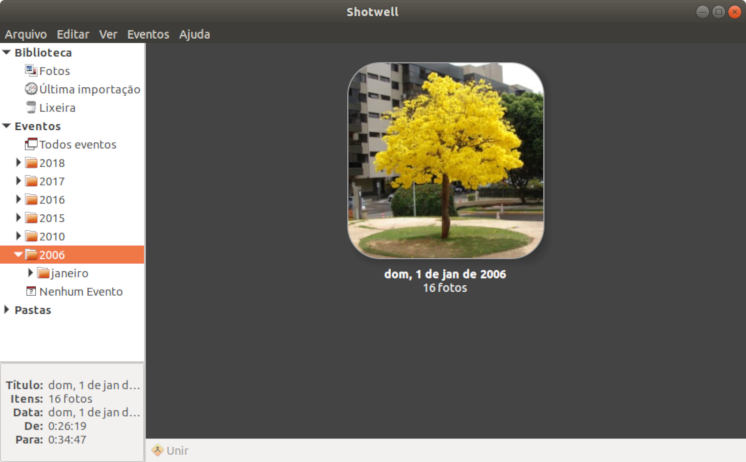
\includegraphics[scale=1.4]{cap03/shotwell.png}
\caption{Shotwell mostrando uma foto que bati em 2006}
\end{figure}
\begin{description}
 \item[Captura de Tela] para quem está escrevendo um livro e precisa tirar alguns \textit{Print Screen} das telas este é o aplicativo ideal, pois entre outras ações ele permite capturar a tela após um intervalo pré-determinado, incluir o cursor ou uma borda na janela parcial. Por padrão esse o aplicativo chamado ao se pressionar as teclas Ctrl + PrintScreen ou Alt + PrintScreen, mas também é possível acessá-lo através do Dash para contar com mais opções de captura.
 \item[EOG] (abreviatura para ``the Eye of Gnome'') é o estranho nome que escolheram para o aplicativo que mostra as imagens por padrão no sistema, ou seja, basta dar um duplo clique na imagem que este aplicativo é chamado, possui os mesmos recursos do visualizador de imagens do Windows.
 \item[Shotwell] Após o adventos das câmeras digitais concorda comigo que manter todas organizadas é uma missão extremamente complicada. A função desse programa é documentar todas as imagens que se encontram no sistema, é possível visualizá-las por ano, publicá-las nas redes sociais (como Facebook ou Picasa) ou mostrá-las em formato de slides.
\end{description}

\subsubsection{Rede e Internet}\index{Padrão do Sistema}
\begin{description}
 \item[Remmina] Que tal acessar um computador a distância e controlá-lo completamente? Calma que não estou falando para se tornar um Hacker, primeiro que teríamos que criar um ``tunelamento'' ou VPN se prefere na rede para em seguida acessá-lo. Esse programa permite o controle total de um computador através da rede.
 \item[Mozilla Firefox] as pessoas possuem um caso de amor ou indiferença ao Firefox (as do segundo grupo geralmente instalam o \textbf{Chrome}), gosto deste navegador principalmente pela possibilidade de inserir diversos plug-ins que me auxiliam nas mais diversas funções – principalmente pela possibilidade de instalar o Selenium para realizar testes automatizados.
 \item[Mozilla Thunderbird] No Windows existe o Outlook (que não está instalado por padrão), só que de todos os clientes de E-mail existentes não troco o Mozilla Thunderbird por nenhum outro. A maior facilidade deste aplicativo consiste na união de várias caixas postais em um aplicativo único além de poder integrá-lo com o Google Calendar e muitos outros aplicativos, o que facilita muito em matéria de organização.
 \item[Contas OnLine] Neste aplicativo é possível incluir e gerenciar suas contas OnLine (Facebook, Google+, Twitter).
 \item[Transmission] Falar de arquivos Torrent parece que estou falando de ``Pirataria'', mas saiba que muitos arquivos grandes da Internet (principalmente imagens ISO) são melhor baixadas nesse formato. Esse é um gerenciador de compartilhamento de arquivos Torrent.
\end{description}

\subsubsection{Utilitários}\index{Padrão do Sistema}
\begin{description}
 \item[Agenda] permite a organização de seus compromissos, lembretes e tarefas através de sua visualização em um calendário mensal ou anual.
 \item[Cheese] permite o controle da WebCam do computador (seja a incorporada do Notebook ou uma externa), bem como gravar de filmes ou tirar fotos – Sim é isso mesmo que está pensando: Say Cheese! Como uma forma de fazer a pessoa sorrir (no Brasil, e só Deus sabe o porquê, usamos: Olha o Passarinho!).
 \item[File Roller] é o gerenciador de arquivos compactados (correspondente ao WinRar) no qual é possível trabalhar com vários modelos de compactação, tais como: 7z, cbr, cbz, iso, jar, rar, tar e zip.
 \item[Caracteres] Smiles é um aplicativo que pode até não ser considerado tão útil, mas com o advento do Whatsapp colocar uma imagem junto com as letras em uma mensagem se tornou um item quase obrigatório, então imagine a situação publicou no Face e deseja colocar um doce ou árvore o que faz?
 \item[Nautilus] é o gerenciador de arquivos e pastas (correspondente ao Windows Explorer), existem alguns atalhos novos para se aprender tais como o uso da tecla Ctrl + T que permite a abertura de uma nova Aba comparar dois diretórios. Cadê o C:? Quem vem do Windows está acostumado com C:, D: ou qualquer outra dessas letras, isso não existe no sistema Linux, são apenas 2 pastas que devemos guardar, sendo que a primeira é a pasta /home que contêm seu usuário e é nesta pasta que colocará seus arquivos, imagens, vídeos ou qualquer outro e a segunda é a pasta / (Computador) no qual estão todas as outras pastas que integram o sistema (que seria a correspondente ao C:) e só podem ser acessadas pelo superusuário.
 \item[Rhythmbox] é um dos mais fantásticos reprodutores de música que conheço (recomendaria até mesmo seu uso no Windows em substituição ao falecido WinAmp) torna possível manter as coleções organizadas bem como acessar Rádios ou Podcasts disponíveis na Internet. Uma das características principais deste aplicativo é a facilidade em se criar as listas de músicas, basta clicar com o botão direito do mouse sobre a música escolhida e selecionar “Adicionar a lista de Reprodução”.
 \item[Totem] é o reprodutor de vídeo padrão (correspondente ao Windows Media Player) pode-se visualizar arquivos de multimídia, como vídeos (com legendas) e músicas, de maneira simples e rápida.
\end{description}

\subsubsection{Jogos}\index{Padrão do Sistema}
\begin{description}
 \item[Mahjongg] possuo esse jogo também no Celular e no Tablet e para mim é um dos melhores quebra-cabeças que conheço, na China é tão popular quanto uma partida de Truco em Goiás.
 \item[Minas] pelo menos se for por causa desse jogo não sentiremos a menor falta do Windows, o objetivo é o mesmo sinalizar o campo minado, e o desafio é o mesmo: Não explodir.
 \item[Paciência AisleRiot] quando migrei para o Linux uma das coisas que mais senti falta foi do ``FreeCell'' e logo de cara fiquei procurando um correspondente na Internet para o Linux. Esse aplicativo já está instalado por padrão e não é o FreeCell, alias não é apenas o ``FreeCell'' pois são mais de 100 jogos do tipo paciência de cartas disponíveis. Basta no menu principal acessar “Alterar Jogo” para ver a lista disponível.
 \item[Sudoku] outro bom jogo de lógica que já vem pré-instalado que consiste (apenas para você que viveu em Plutão nos últimos anos – porém acredito que até lá se jogava isso) de um quebra-cabeça para a ordenação de números em linhas, colunas e casas.
\end{description}

\subsubsection{Gerenciadores do Sistema}\index{Padrão do Sistema}
\begin{description}
 \item[Configurações do Sistema] é uma reunião dos principais aplicativos do Ubuntu que pode ser acessado no menu principal do sistema a direita abaixo do nome do usuário (aonde fica a opção de desligar o sistema), permite as atividades como modificar completamente a aparência visual do sistema, de brilho da tela, janela de bloqueio, impressoras ou rede, suporte a outros idiomas e muitas outras atividades.
 \item[Monitor do Sistema] seria o correspondente a tela de serviços do Windows. Através do monitor é possível verificar os processos que estão em execução, como estão sendo usados os recursos do sistema e as partições do sistema de arquivos.
\end{description}
\section{Atualização do Sistema e do Kernel}\index{Padrão do Sistema}
Uma das coisas que mais me irritava no Windows era a seguinte situação: Já estava no horário para ir dar aula e mandava desligar o Windows, neste momento aparecia a seguinte mensagem assustadora: NÃO DESLIGUE O COMPUTADOR instalando atualização 1 de 1000. Nessa hora minha raiva subia em uma escala de 1 a 100, depois de uns 15 minutos finalmente conseguia desligar o sistema e ir para a escola. Ao chegar na aula com um atraso já mortal e ligar novamente o computador aparece a mensagem matadora: AGUARDE INSTALANDO AS ATUALIZAÇÕES. Juro que me dava vontade de quebrar o computador ali mesmo. Como se ele tivesse sido o culpado pela minha escolha do sistema operacional.

Então o Linux não atualiza? Claro que sim, e constantemente a diferença é que raramente preciso desligar o computador para que as atualizações sejam concluídas. No Linux existe o \textbf{Atualizador de Programas}.
\begin{figure}[H]
\centering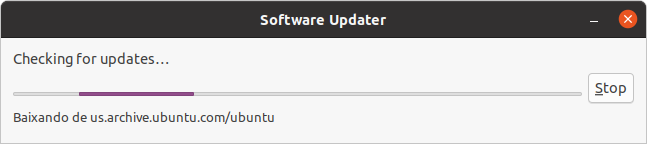
\includegraphics[scale=0.4]{cap03/atualizador.png}
\caption{Atualizador de Programas}
\end{figure}

Só que, normalmente, os usuários Linux tem a mania de ir para uma tela de terminal e digitar: \\
{\ttfamily\$ sudo apt update} \\
{\ttfamily\$ sudo apt upgrade}

O que basicamente realiza o mesmo processo. Esse programa também é ativo temporalmente, ou seja, de quando em quando verifica a necessidade de atualização e APARECE um questionamento SE DESEJA ou NÃO proceder a atualização ao invés de obrigá-lo a ela (como se o sistema nunca mais fosse ligar). Para configurar esse período basta clicar na opção \textbf{Configurações do sistema...} (acessada no canto superior direito abaixo do usuário).

Outra coisa que me perturbava muito no Windows era a atualização de versão, por exemplo, mudou da versão 7 para a 8, é como uma instalação completa para um novo Sistema Operacional (além de ter que pagar tudo novamente), e o pior que tinha me acostumado a isso e achava tudo aquilo um processo muito natural. No Ubuntu tomei um grande susto quando soube que o máximo que tinha de fazer era digitar dois comandos no terminal: \\
{\ttfamily\$ sudo apt update} \\
{\ttfamily\$ sudo apt dist-upgrade}

Após isso era confirmar e esperar, e continuava com meu trabalho normalmente e após terminado o processo a maior diferença estava na opção \textbf{Sobre o Computador} (acessada no canto superior direito abaixo do usuário) que mostrava o número da nova versão do sistema. Para evitar qualquer problema, não tenha dúvida em deixar seu sistema o mais atualizado possível. Fiz isso várias vezes enquanto estava editorando esse livro, e o máximo que acontece? Me mostra a mensagem: "Os softwares foram atualizados e estão em dia". E não "Desliga o computador que preciso finalizar as atualizações".

Então não acontece esse tipo de atualização que precisa desligar? Sim isso ocorre, toda vez que o Kernel do Sistema é modificado. Neste ponto o Ubuntu solicita (e não obriga) que o sistema seja reiniciado, porém bem diferente do que citei no início dessa seção não existe aquela tela: "NÃO DESLIGUE O COMPUTADOR instalando atualização 1 de 1000" pois tudo já está atualizado e é apenas uma questão de reiniciar o computador. Falaremos disso a seguir.

\subsection{Atualização do Kernel}\index{Padrão do Sistema}
Devo confessar que uma das coisas mais interessantes do Linux é que como usuário comecei a me preocupar com detalhes que no Windows estava pouco interessado. Um desses era a versão do Kernel. Devemos lembrar que o \textbf{Linux é o Kernel}, isso significa que passa por atualizações sobre as distros, e estar sempre atualizado é ideal para manter seu sistema saudável principalmente porque falhas são corrigidas.

Um dos blogs que mais consulto e recomendo a todos é o \textbf{Sempre Update}\footnote{Disponível no endereço \url{https://sempreupdate.com.br/}} que contém dicas incríveis e (desculpe o trocadilho) sempre me mantêm atualizado. Para saber qual a versão de seu Kernel, abra uma janela do terminal e digite o seguinte comando: \\
{\ttfamily\$ uname -r}

Manter sempre uma versão estável do Kernel ajuda no suporte, mais dispositivos e componentes, melhor gerenciamento de muitas partes essenciais do sistemas e muitos melhoramentos. A partir da versão 13.10 (\textit{Saucy Salamander}) veio com aplicações 3.8 branch, o que é muito bom para os usuários do GNOME. O que permitiu uma melhor integração com pesquisas online, através de busca no DASH. As configurações de segurança permitem um maior controle sobre o tráfego. 

\subsection{Meus Discos}\index{Padrão do Sistema}
Não tem nada a ver com música e sim os discos do seu computador, no Dash digite Discos e selecione o aplicativo de mesmo nome. Esse aplicativo é bem útil para ver qualquer informação sobre seu HD, unidades de CD e os dispositivos externos. É possível obter diversas informações a respeito de cada uma das unidades apenas selecionando a mesma e pressionando o ícone das engrenagens.
\begin{figure}[H]
\centering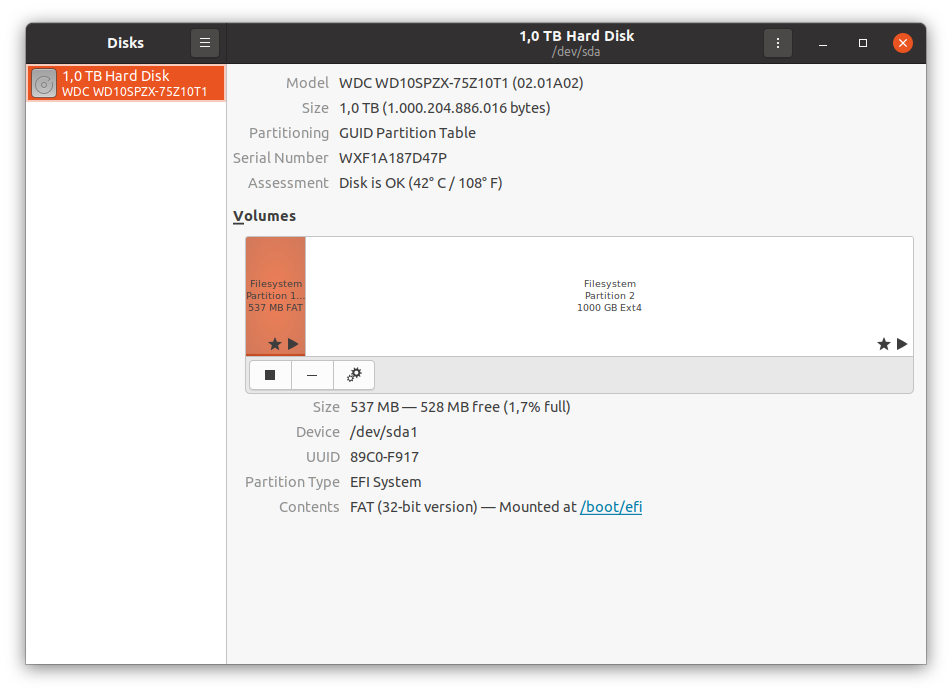
\includegraphics[scale=0.3]{cap03/discos.png}
\caption{Janela do Discos}
\end{figure}

Também é muito útil para formatarmos qualquer dispositivo, por exemplo, insira um pendrive e chame esse aplicativo, selecione a unidade que está localizado seu pendrive e pressione Ctrl + F.

\subsection{Checagem do Disco}\index{Padrão do Sistema}
Um dos comandos que mais conhecia no Windows era \textbf{chkdsk}, isso realiza uma ``checagem dos discos'', qual não foi minha surpresa ao descobrir no Ubuntu esse mesmo comando, bem é um pouquinho diferente mas o propósito é o mesmo. Primeiro passo a fazer é descobrir quais são nossas partições, use o comando: \\
{\ttfamily\$ sudo parted /dev/sda 'print'}

Que mostrará uma lista de todas as partições do sistema, agora podemos realizar uma checagem de qualquer uma dessas partições através do número da mesma com o seguinte comando: \\
{\ttfamily\$ fsck /dev/sda[numero]}

Só que antes de sair correndo e aplicando tais comandos aviso que isso pode CORROMPER seu sistema caso o número informado seja a sua partição atual de trabalho. Então para quê serve isso? Simples, acima expliquei como realizar atualizações do Kernel, pode acontecer de faltar energia entre outras possibilidades e essa atualização ser interrompida. Então existe a possibilidade de corromper o sistema e a única solução conhecida e ter que reinstalar o sistema do zero. Só que existe uma tábua de salvação que é esse comando de checagem, pois esse comando não apenas checa como também corrige seu sistema.

\subsection{O que é Processo Zeitgeist}\index{Padrão do Sistema}
A performance do Ubuntu, nas suas últimas versões, tem sido bastante criticada, principalmente por aqueles usuários que estavam habituados as versões anteriores que eram mais rápidas. Um detalhe que tem afetado a performance é a utilização de um serviço conhecido como Zeitgeist que registra toda sua atividade no Ubuntu.

Este serviço guarda praticamente todas as ações realizadas no Ubuntu, desde qual aplicações que utilizamos a quais arquivos que abrimos. E isto inclui também o que fazemos na Internet, que páginas visitamos, que conversas temos no chat do Ubuntu e que e-mails trocamos.

Essa aplicação se chama \textbf{Privacidade} (o nome do programa verdadeiro é “activity-log-manager”) e é facilmente localizada no Dash ou nas Configurações do Sistema. Para desinstalar o Zeitgeist, abra um terminal e digite os seguintes comando: \\
{\ttfamily\$ sudo apt remove zeitgeist zeitgeist-core zeitgeist-datahub}

Este comando elimina também dependências que não serão mais necessárias. Uma delas é a aplicação ``Privacidade'' (referida acima) e outra é um plugin do reprodutor de músicas ``Rhythmbox'' que ajuda a fazer registo de músicas ouvidas. Além disso as pesquisas das abas do Dash respectivas a Documentos, Vídeos, Músicas, Imagens e Listas de Discussão não mais funcionarão. Uma forma que as pessoas tem feito é instalar um aplicativo chamado \textbf{Activy Log Manager} para tentar controlar as listas, para instalar utilize as seguintes indicações: \vspace{-1em}
\begin{itemize}[noitemsep]
 \item Repositório: zeitgeist/ppa
 \item Aplicativo: activity-log-manager
\end{itemize} 

No Dash chame o aplicativo e configure suas opções. Outra dica é procurar na Loja pelo aplicativo Jornal de Atividades, o Zeitgeist forma listas históricas gigantescas e se  for um usuário desorganizado com seus arquivos o ideal mesmo é desativá-lo. Caso deseje retornar esse serviço, use as seguintes indicações: \vspace{-1em}
\begin{itemize}[noitemsep]
 \item Repositório: zeitgeist/ppa
 \item Aplicativos: zeitgeist zeitgeist-core zeitgeist-datahub \\ activity-log-manager-control-center rhythmbox-plugin-zeitgeist
\end{itemize} 

Não esqueça de reiniciar o Ubuntu.

\section{Ajustes Finos e Serviços Travados}\index{Padrão do Sistema}
Primeiro gosto de deixar meu Ubuntu bem personalizado, tipo colocar a data na barra superior, primeiro precisamos instalar um excelente programa para gerenciar o Gnome, procure na loja por \textbf{Ajustes do Gnome}, ou use o seguinte comando no terminal: \\
{\ttfamily\$ sudo apt install gnome-tweaks}

Acessar o programa e observar que podemos acertar toda a configuração de tela através desse gerenciador. 

Outro detalhe para quem vem do Windows é que com certeza decorou a combinação das teclas Ctrl + Alt + Del e isso fica engraçado no Ubuntu, por padrão essas teclas estão configuradas para encerrar uma sessão. Não pense que o Linux seja maravilhoso e nunca um aplicativo apresenta qualquer problema e não travará, não sei quantas vezes encerrei uma sessão por causa de um aplicativo travado. 

Um aplicativo pode travar em qualquer sistema operacional, ainda não existe esse sistema no qual um aplicativo não trave por qualquer motivo, seja por falta de memória ou por tentar gravar em uma área inválida no HD ou na rede. Resumidamente, fez um I/O (ou E/S em português) está arriscado a travar. 

Existem duas maneiras de destravar um aplicativo, a primeira é abrir um terminal e digitar o comando \textbf{xkill}, no qual o ponteiro do mouse mudará para um alvo e basta apenas clicar na janela bloqueada. A segunda é utilizar o aplicativo \textbf{Monitor do sistema}, só que chamá-lo do Dash pode ser um tanto complicado. Então vamos criar um atalho personalizado para este aplicativo.

No Dash digite: \textbf{Configurações}, agora pesquise por: \textbf{Teclado} (no canto superior esquerdo existe uma Lupa). Clique no botão + no final da lista e na janela do Atalho personalizado digite as seguintes opções: \vspace{-1em}
\begin{itemize}[noitemsep]
 \item Nome: Monitor do sistema
 \item Comando: gnome-system-monitor 
 \item Atalho: Ctrl + Alt + M
\end{itemize}

\subsection{Afinar a Memória Swap e o Cache}\index{Padrão do Sistema}
Em ambiente Unix existe a memória Swap e essa área procura auxiliar uma baixa quantidade de Memória RAM fazendo trocas mais rápidas, ou seja, e a relação entre velocidade de execução dos aplicativos e sua disponibilização em áreas de memória. Podemos ver seu valor padrão de disponibilização através do comando: \\
{\ttfamily\$ sudo cat /proc/sys/vm/swappiness}

A configuração padrão do Ubuntu é feita para servidores, então provavelmente o valor mostrado será 60, esse número varia de 0 a 100. Esse número 60 significa que ao ter abaixo de 60\% de memória livre o sistema envia alguns dados para a partição de SWAP. Ou seja, muitas vezes seu desktop (a menos que seja seu servidor) pode pedir arrego antes de chegar a 60\%, não existe um número ideal para todos, mas vamos começar usando o valor 10 com o seguinte comando: \\
{\ttfamily\$ sudo sysctl -w vm.swappiness=10}

Faça essa alteração e passe um bom tempo realizando suas atividades, veja se está tudo normal e caso contrário aumente gradualmente esse número se sentir necessidade. Ao achar o número ideal, é hora de deixá-lo como padrão do sistema. Editar o arquivo de configuração com o seguinte comando: \\
{\ttfamily\$ sudo gedit /etc/sysctl.conf}

E adicionar uma linha com a seguinte configuração: \textbf{vm.swappiness=[numero encontrado]}. O cache é outra área interessante, responsável por controlar o dinamismo dos swaps do Kernel. Ou seja, ao abrir e fechar um arquivo, pesquisar, visualizar imagens, entre várias outras ações. Primeiro verificar qual é o valor através do seguinte comando: \\
{\ttfamily\$ sudo cat /proc/sys/vm/vfs\_cache\_pressure}

Provavelmente a resposta será 100, o que significa 100\% sobre o desempenho na gestão dos arquivos de discos, se reduzir significa que a RAM terá que trabalhar mais e os processos ficarão mais ágeis no sistema (vale as mesmas observações sobre não existe um valor ideal). Vamos reduzir para 50 com o comando: \\
{\ttfamily\$ sudo sysctl -w vm.vfs\_cache\_pressure=50}

E de modo similar, testar o desempenho do sistema até encontrar o valor correto. Para salvar no arquivo de configuração, adicionar a seguinte linha: \textbf{vm.vfs\_cache\_pressure=[numero encontrado]}. No  \textbf{Monitor do Sistema} aba ``Recursos'' é possível acompanhar como está a disponibilização e o uso das áreas de memória e ajustar o sistema de acordo.

\subsection{Mudando o padrão do Sistema}\index{Padrão do Sistema}
Uma das grandes vantagens em se usar um sistema livre é a possibilidade de poder mudar qualquer chamada do sistema, por exemplo, não gosta do servidor de e-mail padrão? Mude-o. Detesta o editor de textos padrão? Mude-o. Possui um navegador preferido? Troque facilmente para que ele possa ser chamado por padrão. Para fazer isso, no canto superior direito clique na seta para baixo e um menu será aberto:
\begin{figure}[H]
\centering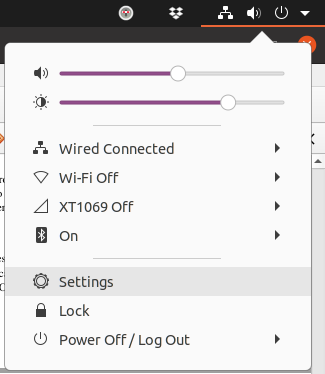
\includegraphics[scale=0.27]{cap03/configura.png}
\caption{Parte dos Ajustes do Sistema}
\end{figure}

Nesta janela podemos aumentar ou diminuir o som ou brilho do sistema, as conexões de rede e bluetooth, ajustes em seu usuário e os três botões do Sistema, que são respectivamente: \vspace{-1em}
\begin{itemize}[noitemsep]
 \item Ajustes de Configuração do Sistema
 \item Bloqueio do Sistema
 \item Desligamento ou reinício do Sistema
\end{itemize}

Na janela de ajustes de Configuração do Sistema é possível modificar os aplicativos que serão chamados como padrão para Web, e-mail, calendário, músicas, vídeos e fotos. Porém, por exemplo, o formato de arquivo PNG que desejamos usar o Gimp por padrão não se encontra aí por ser uma imagem, não se desespere. Localize uma imagem nesse formato através do \textbf{Nautilus} e clique com o botão direito do mouse sobre o arquivo. Selecione a opção \textbf{Propriedades} e a aba ``Abrir com'' e a seguinte janela será mostrada:
\begin{figure}[H]
\centering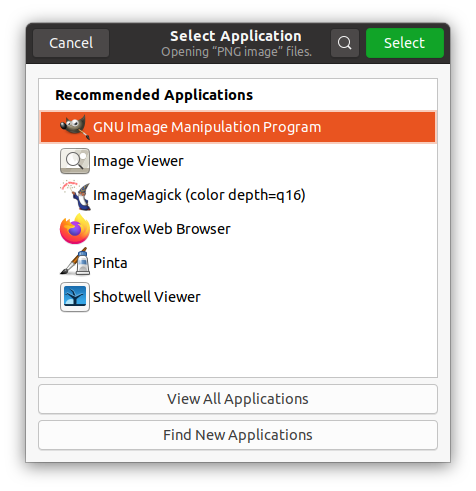
\includegraphics[scale=0.4]{cap03/selecionar.png}
\caption{Selecionar uma Aplicação}
\end{figure}

Agora basta escolher o aplicativo que se deseja para abrir este tipo de arquivo e pressionar o botão \textbf{Definir como padrão}. 

\subsection{Travou? Como sair com segurança}\index{Padrão do Sistema}
Doce sonho quem pensa que é apenas o Windows que trava, isso pode acontecer a qualquer sistema operacional. A ideia é similar a usar \textbf{Ctrl + Alt + Del} porém algumas combinações não derrubam o sistema, mas servem para caso de emergência, para sincronizar os discos ou desligar o computador instantaneamente, evitando que ocorram problemas nos sistemas de arquivos. São as seguintes combinações de teclas: \vspace{-1em}
\begin{itemize}[noitemsep]
 \item \textbf{Alt + Print Screen + O}. Utilizado para desligar o computador rapidamente sem danificar seus sistemas de arquivos, ou quando a máquina trava e por qualquer motivo não permite um desligamento natural através do init. 
 \item \textbf{Alt + Print Screen + B}. Informa ao Kernel do Linux uma chamada de emergência e permite reiniciar a máquina, com a vantagem de sincronizar os discos evitando danos no sistema de arquivos.  
 \item \textbf{Alt + Print Screen + S}. Utilizada para sincronizar discos em caso de emergência. Precisa trabalhar até a ultima hora mas tem medo de danificar seu sistema de arquivo, essa opção sincroniza seus discos.
 \item \textbf{Alt + Print Screen + U}. Se por algum motivo algo está ameaçando a segurança do seu sistema, como a execução acidental de um script malicioso como root ou um programa desconhecido, essa opção coloca os discos em modo somente leitura para evitar danos mais sérios.
\end{itemize}

Outra saída pode ser simplesmente acabar com um processo que está travando seu sistema, matar um processo requer apenas dois comandos no terminal (localizar e matar): \\
{\ttfamily\$ ps -ef | grep [nomeProcesso] \\
\$ sudo kill -9 [pidProcesso]}

\subsection{E agora?}\index{Padrão do Sistema}
Existem vários blogs que mostram o fazer após instalar o sistema operacional Ubuntu, são os chamados acertos no sistema para baixar drivers necessários ou adicionar e configurar alguns programas. Recolhi algumas de suas mais essenciais dicas (ache todos os programas indicados na Loja, a menos que tenha alguma observação contrária).

\subsubsection{Faça 1 – Manter o sistema o mais atualizado possível}\index{Padrão do Sistema}
Acabou de instalar uma nova distribuição ou atualizou o Kernel, durante os próximos 3 dias recomendo que o mais atualizado possível. Isso forçará que qualquer nova correção que aconteceu seja trazida para seu computador, muitas vezes alguns problemas são encontrados logo após a liberação de atualizações e são disponibilizados quase imediatamente.

\subsubsection{Faça 2 – Baixar codecs e outros pacotes extras}\index{Padrão do Sistema}
Para utilizar todo o sistema de multimídia, é preciso instalar alguns codecs e um pequeno conjunto de softwares para tocar DVDs encriptados. Estes itens podem ser encontrados através dos seguintes nomes: \vspace{-1em}
\begin{itemize}[noitemsep]
 \item ubuntu-restricted-extras
 \item libavcodec-extra 
 \item libdvdread4 
\end{itemize}

\subsubsection{Faça 3 – Instalar OpenJava, Compactação RAR e bibliotecas básicas para vídeo}\index{Padrão do Sistema}
Não entendo porque este conjunto já não faz parte da instalação padrão: \\
{\ttfamily\$ sudo apt install openjdk-8-jdk unrar rar libdvd.pkg}

\subsubsection{Faça 4 – Editar Partições}\index{Padrão do Sistema}
\textbf{GParted} é usado para criar, eliminar ou alterar as partições do seu HD, HD Externo e pendrive.

\subsubsection{Faça 5 – Proteger-se com um Firewall}\index{Padrão do Sistema}
\textbf{Gufw} é um firewall muito fácil de usar e bastante eficiente. Para instalar procure na Loja por gufw. Após abrir o programa basta mudar o status para "ON" para deixar seu PC protegido.

\subsubsection{Faça 6 – Personalizar o Ubuntu}\index{Padrão do Sistema}
\textbf{Editor do dconf} é essencial para alguns processos de personalização e funciona como o RegEdit do Windows. Vamos aproveitar para corrigir a barra de atalhos do Nautilus (o Windows Explorer do Linux) onde não é permitida digitar o caminho pois é formada por uma série de botões. O atalho \textbf{Ctrl + L} faria o mesmo efeito, porém gosto de torná-lo padrão, então façamos a seguinte modificação: pesquise no Dash pelo DConf, no painel esquerdo acesse o caminho: org | gnome | nautilus | preferences. Marque a opção: always-use-location-entry.

\subsubsection{Faça 7 – Instale o Twitter no Thunderbird}
Não é necessário ficar entrando no navegador para publicar ou acessar no \textbf{Twitter} é possível adicionar sua conta no gerenciador de e-mails Thunderbird.
\begin{figure}[H]
\centering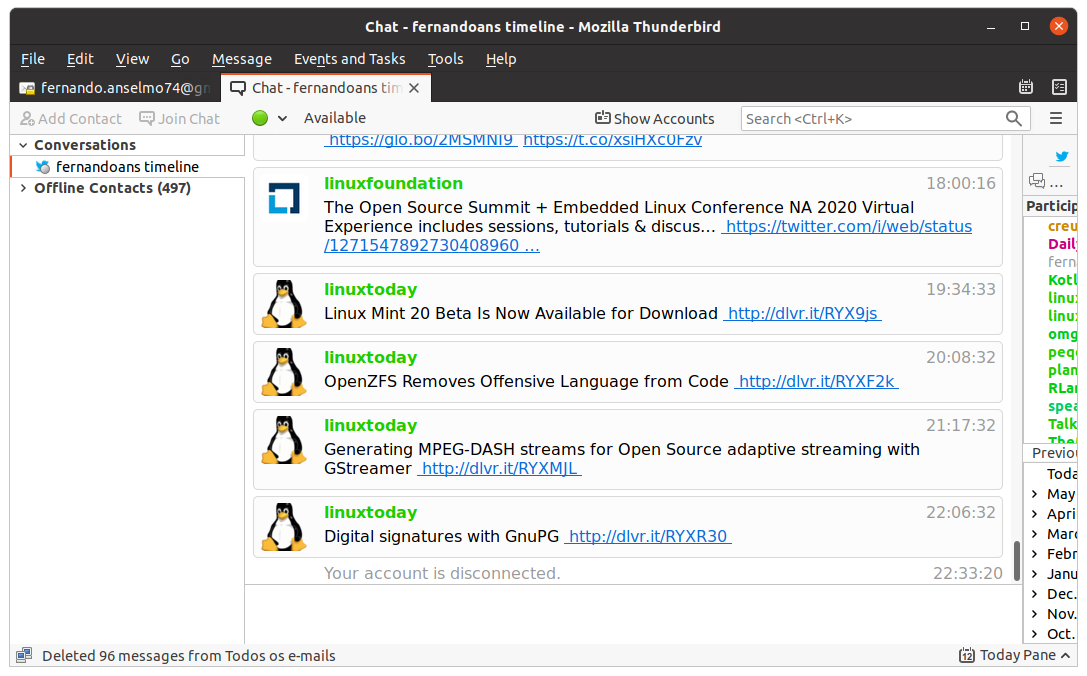
\includegraphics[scale=0.3]{cap03/twitter.png}
\caption{Twitter no Thuderbird}
\end{figure}

\subsubsection{Faça 8 – Usar o Gimp (simplemente o melhor)}\index{Padrão do Sistema}
Uso este programa a muito tempo e tudo o que necessitei realizar com uma imagem o Gimp me atendeu sem o menor problema. Trabalha muito bem com fotos, sobreposição de camadas, composição de imagem e utiliza os mais variados tipos de filtros. E não consigo de modo algum entender porque não vem instalado por padrão no sistema. Fico só pensando o que seria desse livro sem o Gimp, e muitos outros que escrevi.
\begin{figure}[!h]
 \centering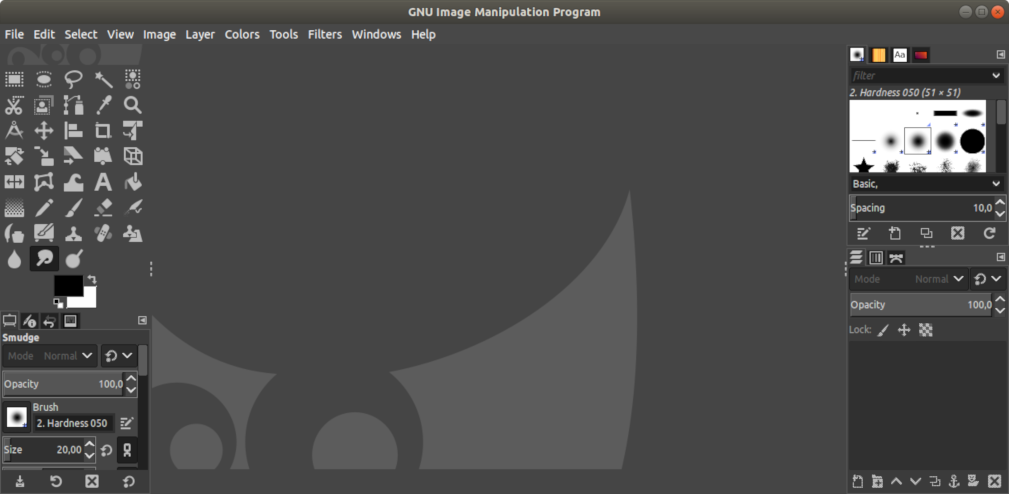
\includegraphics[scale=1.4]{cap03/Gimp.png}
 \caption{Janela do Gimp}
\end{figure} \\
Pode ser encontrado na loja, mas prefiro mantê-lo o mais atualizado possível e a instalação via terminal é muito mais simples: \\
{\ttfamily\$ sudo add-apt-repository ppa:otto-kesselgulasch/gimp} \\
{\ttfamily\$ sudo apt install gimp gimp-gmic gimp-data gimp-data-extras}

\subsubsection{Faça 9 – Aprender R e Assembly}\index{Padrão do Sistema}
Python já é padrão do sistema, segue a instalação de mais duas linguagens que não consigo ficar sem: \\
{\ttfamily\$ sudo apt install nasm \\
\$ sudo apt install r-base}

\subsubsection{Faça 10 – Ter um Antivírus (isso existe?)}
Em qualquer sistema operacional pode-se pegar vírus, isso que não existe vírus para  Linux é loucura, a única diferença é que usuários Linux sabem mais o que estão fazendo e são mais cuidadosos. Além disso, 90\% do planeta usa Windows que não faz a menor distinção entre o superusuário e o usuário normal, então é comum que 99\% dos vírus sejam construídos para esse ambiente. Porém, com o aumento dos usuários Linux, com certeza haverá um aumento da criação de vírus para esse ambiente, então por que não ficar garantido? Procure na Loja por \textbf{clamtk}. \\[3mm]
Está sentindo falta daquelas dicas um monte de outros aplicativos? Não se preocupe na próxima parte deste livro teremos um conjunto dos mais diversos para todos os gostos.

% Final do Capítulo
\clearpage